\chapter{Stereochemistry in Depth}\label{ch:b1:stereochemistry-in-depth}

Crush a few caraway seeds, then a spearmint leaf: two quite different
smells. The main odorant of each is carvone, \ce{C10H14O}, the same atoms
joined in the same order --- but the two carvones are mirror images of
each other, as a left hand is of a right hand, and the receptors of the
nose, themselves built of mirror-asymmetric molecules, tell them apart.
Medicines, flavours and the molecules of life are all built in three
dimensions, and a structural formula that ignores the third dimension
misses half the story. This chapter gives the tools to draw molecules in
space, to name each arrangement without ambiguity, to follow the
rotations that molecules perform constantly, and to measure the one
physical property that tells mirror images apart.

\begin{recall}
The school volume (grade 12) introduced \omterm{def:b1:stereochemistry-in-depth:stereocentre}{chiral} molecules, the asymmetric
carbon, \omterm{def:b1:stereochemistry-in-depth:enantiomers}{enantiomers}, $Z$/$E$ isomers and the \omterm{def:b1:stereochemistry-in-depth:isomers}{conformations} of ethane.
The tetrahedral arrangement of four bonds around carbon and the
$\sigma$/$\pi$ description of single and double bonds come from
\cref{ch:b1:lewis-resonance-vsepr}.
\end{recall}

\begin{omfigure}
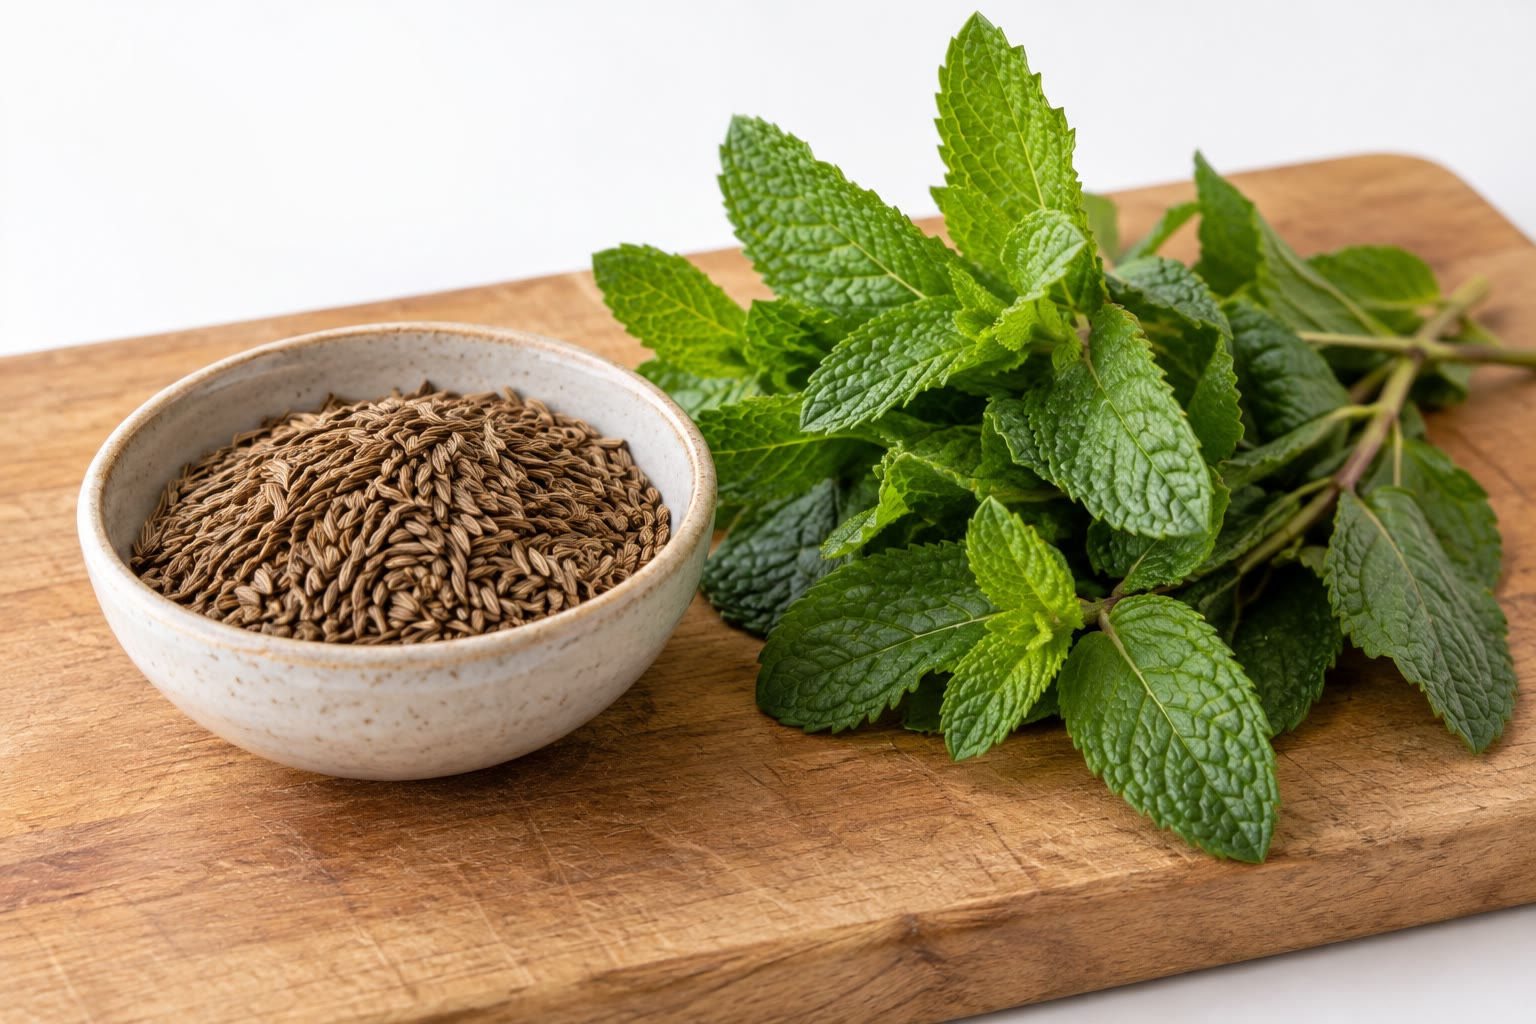
\includegraphics[width=0.55\linewidth]{images/book2/ai/b1-16-caraway-mint.jpg}

{\small Caraway seeds and spearmint leaves. Caraway owes its smell mainly
to \cip{S}-carvone, spearmint to its mirror image, \cip{R}-carvone.}
\end{omfigure}

\section{Isomers and representations}

\begin{definition}[Constitution, configuration, conformation]\label{def:b1:stereochemistry-in-depth:isomers}
Two compounds of the same formula whose atoms are joined in a different
order are \emph{constitutional isomers}\index{constitutional isomers}.
Compounds with the same constitution whose atoms differ only in their
arrangement in space are \emph{stereoisomers}\index{stereoisomers}. The
arrangement that can be changed only by breaking bonds is the
\emph{configuration}\index{configuration} of a stereoisomer; an
arrangement obtained by rotation about single bonds, without breaking any,
is a \emph{conformation}\index{conformation}.
\end{definition}

At room temperature, rotations about single bonds take place billions of
times a second: \omterm{def:b1:stereochemistry-in-depth:isomers}{conformations} interconvert and cannot be isolated, while
\omterm{def:b1:stereochemistry-in-depth:isomers}{configurations} are stable and give distinct compounds.

\begin{definition}[Representations]\label{def:b1:stereochemistry-in-depth:representations}
In the \emph{Cram representation}\index{Cram representation} two bonds
are drawn in the plane of the page, a solid wedge points towards the
reader and a hashed wedge away. A \emph{Newman projection}\index{Newman projection}
views a molecule along one C--C bond: the front carbon is a
point where its three other bonds meet, the rear carbon a circle from
whose rim its bonds emerge. In a \emph{Fischer projection}\index{Fischer projection}
the carbon chain is vertical, horizontal bonds point towards
the reader and vertical bonds away; each crossing is a stereogenic carbon.
\end{definition}

\begin{omfigure}
\begin{tikzpicture}[font=\small]
  % staggered and eclipsed ethane, Newman
  \pic (s) at (0,0) {omnewman={90}{30}};
  \foreach \k in {1,2,3} { \node at (s-f\k) {H}; \node at (s-b\k) {H}; }
  \node at (0,-1.9) {staggered};
  \pic (e) at (3.6,0) {omnewman={90}{108}};
  \foreach \k in {1,2,3} { \node at (e-f\k) {H}; }
  \foreach \k in {1,2,3} { \node[font=\scriptsize, black!60] at ($(e-b\k)!-0.12!(e-c)$) {H}; }
  \node at (3.6,-1.9) {eclipsed};
  % Fischer projection of (R)-lactic acid
  \begin{scope}[xshift=7.6cm]
    \draw[thick] (-0.9,0) -- (0.9,0) (0,-0.9) -- (0,0.9);
    \node[above] at (0,0.9) {\ce{COOH}};
    \node[below] at (0,-0.9) {\ce{CH3}};
    \node[left] at (-0.9,0) {H};
    \node[right] at (0.9,0) {OH};
    \node at (0,-1.9) {Fischer};
  \end{scope}
  % Cram of the same
  \begin{scope}[xshift=11.0cm]
    \node at (0,0) {\chemfig{C(-[2]COOH)(-[:210]H_3C)(<:[:-12]OH)(<[:-55]H)}};
    \node at (0,-1.9) {Cram};
  \end{scope}
\end{tikzpicture}

{\small Left: \omterm{def:b1:stereochemistry-in-depth:representations}{Newman projections} of ethane along its C--C bond, staggered
(rear bonds between the front ones) and eclipsed (rear bonds hidden
behind the front ones, drawn slightly offset). Right: the same molecule,
\cip{R}-lactic acid, as a \omterm{def:b1:stereochemistry-in-depth:representations}{Fischer projection} and in \omterm{def:b1:stereochemistry-in-depth:representations}{Cram representation}
(the vertical bonds of the Fischer cross point away from the reader, the
horizontal ones towards the reader).}
\end{omfigure}

\begin{method}[From Cram to Newman]\label{met:b1:stereochemistry-in-depth:newman-from-cram}
\begin{enumerate}
  \item Choose the bond to look along and the end nearer to the eye.
  \item Draw the three bonds of the front carbon from the centre,
        keeping their order (clockwise or anticlockwise) as seen from the
        eye.
  \item Draw the rear carbon's bonds from the circle, with their order as
        seen from the same side.
  \item Check: rotating the rear carbon by $60^\circ$ passes from
        staggered to eclipsed; by $120^\circ$, from one \omterm{def:b1:stereochemistry-in-depth:conformations}{staggered
        conformation} to the next.
\end{enumerate}
\end{method}

\section{Configuration: the CIP rules}

\begin{definition}[CIP rules, descriptors]\label{def:b1:stereochemistry-in-depth:cip}
The \emph{CIP rules}\index{CIP rules} (Cahn--Ingold--Prelog) rank the four
substituents of a \omterm{def:b1:stereochemistry-in-depth:stereocentre}{stereogenic centre}: higher atomic number first; on a
tie, compare the sets of atoms attached next, and so on outwards; a
double bond counts as two single bonds to duplicated atoms. With the
lowest-ranked substituent pointing away from the eye, the sequence
$1 \to 2 \to 3$ turning clockwise defines the descriptor \cip{R}, and
anticlockwise \cip{S}. For a double bond with two substituents on each
carbon, \cip{Z} means the two higher-ranked ones are on the same side and
\cip{E} on opposite sides.
\end{definition}

\begin{method}[Assigning \texorpdfstring{\cip{R}}{(R)} or \texorpdfstring{\cip{S}}{(S)}]\label{met:b1:stereochemistry-in-depth:cip}
\begin{enumerate}
  \item Rank the four substituents by the \omterm{def:b1:stereochemistry-in-depth:cip}{CIP rules}.
  \item If the lowest-ranked one points away from you (hashed wedge, or a
        vertical bond of a \omterm{def:b1:stereochemistry-in-depth:representations}{Fischer projection}), read the turn of
        $1 \to 2 \to 3$ directly.
  \item If it points towards you (solid wedge, horizontal Fischer bond),
        read the turn and reverse the descriptor.
  \item Exchanging any two substituents reverses the descriptor: a quick
        check.
\end{enumerate}
In lactic acid, $\ce{OH} > \ce{COOH} > \ce{CH3} > \ce{H}$ (O; then C(O,O,O)
beats C(H,H,H)). In the \omterm{def:b1:stereochemistry-in-depth:representations}{Fischer projection} above, H is horizontal
(towards us) and $\ce{OH} \to \ce{COOH} \to \ce{CH3}$ turns anticlockwise:
reversed, the centre is \cip{R}.
\end{method}

\section{Chirality and its consequences}

\begin{definition}[Stereogenic centre, chirality]\label{def:b1:stereochemistry-in-depth:stereocentre}
An object is \emph{chiral}\index{chiral} if it cannot be superposed on its
mirror image, \emph{achiral}\index{achiral} otherwise; the property is
\emph{chirality}\index{chirality}. A \emph{stereogenic
centre}\index{stereogenic centre} is an atom at which exchanging two
substituents gives a stereoisomer; a tetrahedral carbon with four
different substituents is one.
\end{definition}

A molecule with a plane of symmetry or a centre of symmetry is \omterm{def:b1:stereochemistry-in-depth:stereocentre}{achiral};
a molecule with neither is \omterm{def:b1:stereochemistry-in-depth:stereocentre}{chiral} in practice. The exact criterion, in
terms of symmetry operations, is given in the Year~3 volume.

\begin{definition}[Enantiomers, diastereomers, meso compound, racemic mixture]\label{def:b1:stereochemistry-in-depth:enantiomers}
Two \omterm{def:b1:stereochemistry-in-depth:isomers}{stereoisomers} that are mirror images of each other are
\emph{enantiomers}\index{enantiomers}; \omterm{def:b1:stereochemistry-in-depth:isomers}{stereoisomers} that are not are
\emph{diastereomers}\index{diastereomers}. A \emph{meso
compound}\index{meso compound} has \omterm{def:b1:stereochemistry-in-depth:stereocentre}{stereogenic centres} but is \omterm{def:b1:stereochemistry-in-depth:stereocentre}{achiral}. An
equimolar mixture of two enantiomers is a \emph{racemic
mixture}\index{racemic mixture}.
\end{definition}

\begin{proposition}[Number of stereoisomers]\label{prop:b1:stereochemistry-in-depth:max-stereoisomers}
A molecule with $n$ \omterm{def:b1:stereochemistry-in-depth:stereocentre}{stereogenic centres} (and no other stereogenic unit)
has at most $2^n$ \omterm{def:b1:stereochemistry-in-depth:isomers}{stereoisomers}, in at most $2^{n-1}$ pairs of
\omterm{def:b1:stereochemistry-in-depth:enantiomers}{enantiomers}; meso forms make the number smaller.
\end{proposition}

\begin{proof}
Each centre is \cip{R} or \cip{S} independently: $2^n$ combinations. The
mirror image changes every descriptor, so the combinations pair up into
\omterm{def:b1:stereochemistry-in-depth:enantiomers}{enantiomers}, $2^{n-1}$ pairs. If a combination is its own mirror image
after a rotation of the molecule (a meso form), its pair collapses into
one compound.
\end{proof}

Tartaric acid, \ce{HOOC-CH(OH)-CH(OH)-COOH}, has two equivalent centres:
\cip{R,R} and \cip{S,S} are \omterm{def:b1:stereochemistry-in-depth:enantiomers}{enantiomers}, while \cip{R,S} has a mirror
plane between the two carbons and is meso: three \omterm{def:b1:stereochemistry-in-depth:isomers}{stereoisomers}, not four.

\begin{proposition}[Properties of enantiomers]\label{prop:b1:stereochemistry-in-depth:enantiomer-properties}
Two \omterm{def:b1:stereochemistry-in-depth:enantiomers}{enantiomers} have the same melting and boiling points, solubilities
in \omterm{def:b1:stereochemistry-in-depth:stereocentre}{achiral} solvents, spectra and reactivity towards \omterm{def:b1:stereochemistry-in-depth:stereocentre}{achiral} reagents;
they differ in their action on polarised light and in their interactions
with other \omterm{def:b1:stereochemistry-in-depth:stereocentre}{chiral} molecules. \omterm{def:b1:stereochemistry-in-depth:enantiomers}{Diastereomers} differ in all their
properties.
\end{proposition}

\begin{proof}
Every property that depends only on distances and angles inside the
molecule, or between it and \omterm{def:b1:stereochemistry-in-depth:stereocentre}{achiral} partners, is the same for an object
and its mirror image, since a reflection preserves distances and
angles. A \omterm{def:b1:stereochemistry-in-depth:stereocentre}{chiral} partner (a receptor, a \omterm{def:b1:stereochemistry-in-depth:stereocentre}{chiral} reagent, the helical path
of polarised light described below) makes pairs that are diastereomeric,
no longer mirror images, which therefore differ. \omterm{def:b1:stereochemistry-in-depth:enantiomers}{Diastereomers} are not
related by any reflection: their internal distances differ.
\end{proof}

\begin{omfigure}
\begin{tikzpicture}[font=\small, line join=round]
  \foreach \dx/\kind/\lab in {0/1/{\cip{R}-carvone (spearmint)}, 5.2/0/{\cip{S}-carvone (caraway)}} {
  \begin{scope}[xshift=\dx cm]
    \coordinate (c1) at (0,1); \coordinate (c2) at (0.87,0.5);
    \coordinate (c3) at (0.87,-0.5); \coordinate (c4) at (0,-1);
    \coordinate (c5) at (-0.87,-0.5); \coordinate (c6) at (-0.87,0.5);
    \draw[thick] (c1) -- (c2) -- (c3) -- (c4) -- (c5) -- (c6) -- cycle;
    \draw[thick] ($(c2)!0.15!(c3)+(-0.12,0)$) -- ($(c3)!0.15!(c2)+(-0.12,0)$);
    \draw[thick] (c1) -- ++(0,0.7) node[above] {O};
    \draw[thick] ($(c1)+(0.1,0)$) -- ++(0,0.62);
    \draw[thick] (c2) -- ++(0.75,0.43) node[right] {\ce{CH3}};
    \coordinate (q) at ($(c5)+(-0.75,-0.43)$);
    \ifnum\kind=1
      \fill (c5) -- ($(q)+(0.06,-0.1)$) -- ($(q)+(-0.06,0.1)$) -- cycle;
    \else
      \foreach \t in {0.15,0.3,0.45,0.6,0.75,0.9}
        \draw ($(c5)!\t!(q)+(\t*0.06,-\t*0.1)$) -- ($(c5)!\t!(q)+(-\t*0.06,\t*0.1)$);
    \fi
    \draw[thick] (q) -- ++(-0.6,0.5) node[above] {\ce{CH2}};
    \draw[thick] ($(q)+(0.08,0.06)$) -- ++(-0.6,0.5);
    \draw[thick] (q) -- ++(0,-0.75) node[below] {\ce{CH3}};
    \node[font=\scriptsize] at ($(c5)+(0.35,0.12)$) {5};
    \node at (0,-2.85) {\lab};
  \end{scope}}
\end{tikzpicture}

{\small The two carvones, drawn on the same skeleton: the isopropenyl group
on C5 points towards the reader (solid wedge) in one and away from the
reader (hashed wedge) in the other, the hydrogen of C5 (not drawn) on the
opposite side. They are mirror images of each other: \omterm{def:b1:stereochemistry-in-depth:enantiomers}{enantiomers}
(\cref{exo:b1:stereochemistry-in-depth:4}).}
\end{omfigure}

\begin{history}[A tetrahedral carbon]
\begin{minipage}[t]{0.2\linewidth}\vspace{0pt}
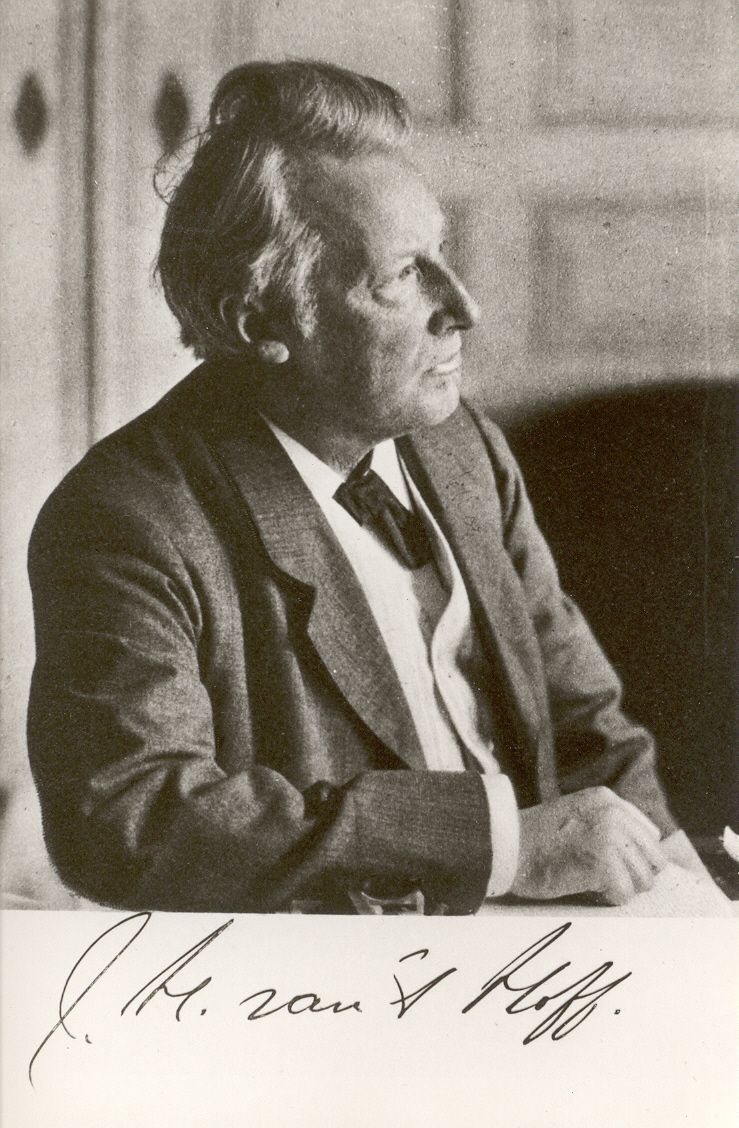
\includegraphics[width=\linewidth]{images/book2/van-t-hoff.jpg}
\end{minipage}\hfill
\begin{minipage}[t]{0.76\linewidth}\vspace{0pt}
Jacobus Henricus van 't Hoff proposed, as a young chemist, that the four
bonds of a carbon atom point to the corners of a tetrahedron. A carbon
with four different substituents then exists as two mirror-image
arrangements, which explained why some compounds come in two forms that
differ only in the way they rotate polarised light. The idea is the
starting point of every drawing in this chapter.
(Photograph published in 1911, public domain, Wikimedia Commons.)
\end{minipage}
\end{history}

\section{Conformations}

\begin{definition}[Torsion angle and conformations]\label{def:b1:stereochemistry-in-depth:conformations}
For four atoms A--B--C--D, the \emph{torsion angle}\index{torsion angle}
$\theta$ about B--C is the angle between the planes ABC and BCD, read on a
\omterm{def:b1:stereochemistry-in-depth:representations}{Newman projection} along B--C. A \omterm{def:b1:stereochemistry-in-depth:isomers}{conformation} is an \emph{eclipsed
conformation}\index{eclipsed conformation} when the bonds of the front
and rear carbons are aligned in projection, a \emph{staggered
conformation}\index{staggered conformation} when they alternate. In
butane, viewed along C2--C3, the staggered \omterm{def:b1:stereochemistry-in-depth:isomers}{conformation} with the two
methyl groups at $180^\circ$ is the \emph{anti conformation}\index{anti conformation},
those at $\pm 60^\circ$ are \emph{gauche
conformations}\index{gauche conformation}. In cyclohexane, the
strain-free puckered ring is the \emph{chair}\index{chair}; each carbon
carries one \emph{axial}\index{axial} bond, parallel to the ring's
axis, and one \emph{equatorial}\index{equatorial} bond, roughly in the
ring's mean plane. The \emph{ring flip}\index{ring flip} converts one
chair into the other, every axial bond becoming equatorial and the
reverse.
\end{definition}

\begin{omfigure}
\begin{tikzpicture}
\begin{axis}[
  width=0.82\linewidth, height=5.8cm, xmin=0, xmax=360, ymin=0, ymax=21,
  legend style={font=\scriptsize, draw=none, at={(0.5,0.62)}, anchor=center},
  axis x line=bottom, axis y line=left, xlabel={torsion angle $\theta$ (degrees)},
  ylabel={energy (kJ/mol)}, xtick={0,60,120,180,240,300,360},
  tick label style={font=\small}, label style={font=\small}]
\addplot[omDef, very thick] table[x=theta, y=butane] {figdata/out/bachelor-1-butane-torsion.dat};
\addplot[omProp, thick, dashed] table[x=theta, y=ethane] {figdata/out/bachelor-1-butane-torsion.dat};
\node[font=\scriptsize, anchor=south west] at (axis cs:0,18.4) {syn};
\node[font=\scriptsize, anchor=south] at (axis cs:62,18.4) {gauche};
\node[font=\scriptsize, anchor=south] at (axis cs:120,18.4) {eclipsed};
\node[font=\scriptsize, anchor=south] at (axis cs:180,18.4) {anti};
\node[font=\scriptsize, anchor=south] at (axis cs:240,18.4) {eclipsed};
\node[font=\scriptsize, anchor=south] at (axis cs:298,18.4) {gauche};
\node[font=\scriptsize, anchor=south east] at (axis cs:360,18.4) {syn};
\legend{butane, ethane}
\end{axis}
\end{tikzpicture}

{\small Torsional energy of butane about its central bond (solid; $\theta
= 0$ when the methyl groups eclipse each other) and of ethane (dashed),
computed from experimental torsional potentials. Ethane: barrier
\qty{12.2}{kJ/mol}. Butane: anti most stable; gauche \qty{2.8}{kJ/mol}
higher, at $\theta = 62^\circ$; barriers \qty{15.2}{kJ/mol} (methyl
eclipsing hydrogen) and \qty{16.5}{kJ/mol} (methyl eclipsing methyl).}
% ledger: rot:ethane-V3, rot:butane-V1, rot:butane-V2, rot:butane-V3, rot:butane-V4, rot:butane-V5, rot:butane-V6 (curves in figdata/bachelor-1/butane-torsion.py)
\end{omfigure}

The barriers are small compared with the thermal energy available in
collisions ($RT = \qty{2.5}{kJ/mol}$ at room temperature, and much more in
the tail of the distribution, \cref{ch:b1:elementary-steps}): rotation is
fast, and butane is a mixture of anti and gauche molecules that cannot be
separated.

\begin{method}[Drawing a chair]\label{met:b1:stereochemistry-in-depth:draw-chair}
\begin{enumerate}
  \item Draw two parallel lines slanting slightly downwards to the right,
        offset; join their ends with a V at the left and an inverted V at
        the right to close the six-membered ring.
  \item \omterm{def:b1:stereochemistry-in-depth:conformations}{Axial} bonds are vertical: up on the carbons that point up, down on
        those that point down, alternating round the ring.
  \item \omterm{def:b1:stereochemistry-in-depth:conformations}{Equatorial} bonds are parallel to the ring bonds once removed, and
        point outwards.
  \item To flip the ring, draw the other \omterm{def:b1:stereochemistry-in-depth:conformations}{chair}; a substituent \omterm{def:b1:stereochemistry-in-depth:conformations}{axial} on one
        is \omterm{def:b1:stereochemistry-in-depth:conformations}{equatorial} on the other.
\end{enumerate}
\end{method}

\begin{omfigure}
\begin{tikzpicture}[font=\small]
  \pic (a) at (0,0) {omchair};
  \foreach \k in {1,2,3,4,5,6} \draw[omProp, thick] (a-c\k) -- (a-a\k);
  \foreach \k in {1,2,3,4,5,6} \draw[omDef, thick] (a-c\k) -- (a-e\k);
  \node[omProp, anchor=south] at (a-a3) {axial};
  \node[omDef, anchor=north] at (a-e5) {equatorial};
  \begin{scope}[xshift=4.9cm]
    \pic (b) at (0,0) {omchair};
    \draw[thick] (b-c1) -- (b-e1) node[right] {\ce{CH3}};
    \draw[thick] (b-c1) -- (b-a1) node[above] {H};
    \node at (0,-1.5) {equatorial \ce{CH3}};
  \end{scope}
  \draw[<->, thick] (8.1,0) -- (8.8,0) node[midway, above] {flip};
  \begin{scope}[xshift=10.45cm]
    \pic (c) at (0,0) {omchairflip};
    \draw[thick] (c-c4) -- (c-a4) node[below] {\ce{CH3}};
    \draw[thick] (c-c4) -- (c-e4) node[right] {H};
    \node at (0,-1.5) {axial \ce{CH3}};
  \end{scope}
\end{tikzpicture}

{\small Left: the \omterm{def:b1:stereochemistry-in-depth:conformations}{chair} of cyclohexane with its six \omterm{def:b1:stereochemistry-in-depth:conformations}{axial} bonds (orange,
alternately up and down) and six \omterm{def:b1:stereochemistry-in-depth:conformations}{equatorial} bonds (blue). Right: the two
\omterm{def:b1:stereochemistry-in-depth:conformations}{chairs} of methylcyclohexane, interconverted by the \omterm{def:b1:stereochemistry-in-depth:conformations}{ring flip}; the methyl
group is \omterm{def:b1:stereochemistry-in-depth:conformations}{equatorial} in one, \omterm{def:b1:stereochemistry-in-depth:conformations}{axial} in the other.}
\end{omfigure}

\begin{proposition}[Equatorial substituents are preferred]\label{prop:b1:stereochemistry-in-depth:chair-substituent}
In a monosubstituted cyclohexane the \omterm{def:b1:stereochemistry-in-depth:conformations}{chair} with the substituent
\omterm{def:b1:stereochemistry-in-depth:conformations}{equatorial} is the more stable. For a methyl group, the axial position adds
two gauche interactions with ring carbons, each worth that of butane
(\qtyrange{2.8}{2.9}{kJ/mol}), about \qty{5.7}{kJ/mol} in all: an estimate
of the energy difference.
\end{proposition}

\begin{proof}
Viewed along the C1--C2 bond, an \omterm{def:b1:stereochemistry-in-depth:conformations}{axial} methyl on C1 is gauche to C3 of
the ring; viewed along C1--C6, gauche to C5: two gauche butane-like
interactions, which are also seen as the crowding of the methyl with the
\omterm{def:b1:stereochemistry-in-depth:conformations}{axial} hydrogens on C3 and C5 (the 1,3-diaxial interactions). An
\omterm{def:b1:stereochemistry-in-depth:conformations}{equatorial} methyl is anti to C3 and C5. Each gauche interaction costs
what it costs in butane, \qty{2.8}{kJ/mol} in the torsional potential of
the figure.
\end{proof}

With $\Delta E = \qty{5.7}{kJ/mol}$, the ratio of \omterm{def:b1:stereochemistry-in-depth:conformations}{equatorial} to \omterm{def:b1:stereochemistry-in-depth:conformations}{axial}
\omterm{def:b1:stereochemistry-in-depth:conformations}{chairs} at \qty{25}{\celsius} is $\exp(\Delta E/RT) = 10$: about
\qty{91}{\percent} \omterm{def:b1:stereochemistry-in-depth:conformations}{equatorial} (\cref{exo:b1:stereochemistry-in-depth:9}).
Large groups, such as tert-butyl, lock the ring in the \omterm{def:b1:stereochemistry-in-depth:conformations}{chair} where they
are \omterm{def:b1:stereochemistry-in-depth:conformations}{equatorial}.

\section{Optical activity}

\begin{definition}[Optical activity, specific rotation]\label{def:b1:stereochemistry-in-depth:optical-activity}
A substance shows \emph{optical activity}\index{optical activity} if it
rotates the plane of polarisation of linearly polarised light passing
through it. Seen by an observer facing the light, a
\emph{dextrorotatory}\index{dextrorotatory} substance, written $(+)$,
rotates it clockwise, a \emph{laevorotatory}\index{laevorotatory} one,
$(-)$, anticlockwise. The \emph{specific rotation}\index{specific rotation}
is $[\alpha] = \alpha/(\ell c)$, where $\alpha$ is the measured
angle in degrees, $\ell$ the path length in decimetres and $c$ the mass
concentration in \unit{g/mL}; it depends on the wavelength (usually the
yellow sodium line), the temperature and the solvent.
\end{definition}

\begin{omfigure}
\begin{tikzpicture}[font=\small, >={Stealth}]
  \fill[yellow!70!orange] (0,0) circle (0.25);
  \node[below] at (0,-0.45) {lamp};
  \draw[thick] (1.3,-0.7) rectangle (1.45,0.7); \node[below] at (1.37,-0.75) {polariser};
  \draw[omDef!20, fill=omDef!10] (2.4,-0.45) rectangle (5.6,0.45);
  \node at (4.0,0) {sample, length $\ell$};
  \draw[thick] (6.5,-0.7) rectangle (6.65,0.7); \node[below] at (6.57,-0.75) {analyser};
  \draw (7.6,0) circle (0.3); \node[below] at (7.6,-0.45) {eye};
  \draw[->, orange!80!black] (0.3,0) -- (1.25,0);
  \draw[->, orange!80!black] (1.5,0) -- (2.35,0);
  \draw[->, orange!80!black] (5.65,0) -- (6.45,0);
  % polarisation planes
  \draw[thick, omThm] (1.9,-0.35) -- (1.9,0.35);
  \draw[thick, omThm] (6.05,-0.33) -- ++(70:0.0) -- (5.93,0.33);
  \draw[->, omThm] (5.75,0.55) arc[start angle=100, end angle=70, radius=0.6];
  \node[omThm, above] at (6.1,0.75) {$\alpha$};
\end{tikzpicture}

{\small A polarimeter. The polariser lets through light vibrating in one
plane; the \omterm{def:b1:stereochemistry-in-depth:stereocentre}{chiral} sample rotates that plane by $\alpha$; the analyser is
turned until the light is extinguished again, which measures $\alpha$.}
\end{omfigure}

\begin{proposition}[Biot's law]\label{prop:b1:stereochemistry-in-depth:biot}
For a dilute solution of several optically active solutes, the angle of
rotation is additive, $\alpha = \ell\sum_i [\alpha]_i c_i$ (\emph{Biot's
law}\index{Biot's law}). Two \omterm{def:b1:stereochemistry-in-depth:enantiomers}{enantiomers} have opposite \omterm{def:b1:stereochemistry-in-depth:optical-activity}{specific
rotations}; a \omterm{def:b1:stereochemistry-in-depth:enantiomers}{racemic mixture} does not rotate light.
\end{proposition}

\begin{proof}
Each solute contributes independently in dilute solution, in proportion
to the number of molecules crossed, that is to $\ell c_i$; this is the
experimental content of the law. A reflection changes clockwise into
anticlockwise: the mirror-image molecule rotates the plane by the opposite
angle, and in a \omterm{def:b1:stereochemistry-in-depth:enantiomers}{racemic mixture} the two contributions cancel.
\end{proof}

For a mixture of two \omterm{def:b1:stereochemistry-in-depth:enantiomers}{enantiomers} at total concentration $c$, the fraction
$x$ of the $(-)$ form gives $\alpha = \ell c[\alpha]_{(-)}(x - (1 - x)) =
\ell c[\alpha]_{(-)}(2x - 1)$: measuring $\alpha$ gives the composition.
Optical rotation is not linked in any simple way to the descriptor: an
\cip{R} compound may be $(+)$ or $(-)$; spearmint's \cip{R}-carvone is
\omterm{def:b1:stereochemistry-in-depth:optical-activity}{laevorotatory}.

\section{Exercises}

\begin{exercise}[$\star$]\label{exo:b1:stereochemistry-in-depth:1}
Classify each pair as \omterm{def:b1:stereochemistry-in-depth:isomers}{constitutional isomers}, \omterm{def:b1:stereochemistry-in-depth:enantiomers}{enantiomers}, \omterm{def:b1:stereochemistry-in-depth:enantiomers}{diastereomers}
or two \omterm{def:b1:stereochemistry-in-depth:isomers}{conformations} of one compound: butan-1-ol and butan-2-ol;
\cip{R}- and \cip{S}-butan-2-ol; \cip{Z}- and \cip{E}-but-2-ene; the anti
and \omterm{def:b1:stereochemistry-in-depth:conformations}{gauche conformations} of butane; \cip{R,R}- and \cip{R,S}-tartaric
acid.
\end{exercise}

\begin{exercise}[$\star$]\label{exo:b1:stereochemistry-in-depth:2}
Rank by the \omterm{def:b1:stereochemistry-in-depth:cip}{CIP rules}: \ce{-OH}, \ce{-NH2}, \ce{-CH3}, \ce{-H}; then
\ce{-CH2OH}, \ce{-CHO}, \ce{-COOH}, \ce{-CH(CH3)2}; then \ce{-Cl},
\ce{-CH2Cl}, \ce{-CCl3}, \ce{-Br}.
\end{exercise}

\begin{exercise}[$\star$]\label{exo:b1:stereochemistry-in-depth:3}
How many \omterm{def:b1:stereochemistry-in-depth:isomers}{stereoisomers} have 2,3-dichlorobutane, 2-bromo-3-chlorobutane
and pentane-2,4-diol? Identify the meso forms.
\end{exercise}

\begin{exercise}[$\star$]\label{exo:b1:stereochemistry-in-depth:4}
Rank the four substituents of C5 of carvone by the \omterm{def:b1:stereochemistry-in-depth:cip}{CIP rules} and check
the descriptors given in the figure of the two carvones (solid wedge:
the isopropenyl group towards the reader, H away).
\end{exercise}

\begin{exercise}[$\star\star$]\label{exo:b1:stereochemistry-in-depth:5}
Draw the \omterm{def:b1:stereochemistry-in-depth:representations}{Newman projections} of butane along C2--C3 at $\theta = 0$, 60,
120 and $180^\circ$ and read their energies on the curve. What fraction of
the molecules would be gauche if the gauche and anti energies were equal?
\end{exercise}

\begin{exercise}[$\star\star$]\label{exo:b1:stereochemistry-in-depth:6}
Draw the \omterm{def:b1:stereochemistry-in-depth:representations}{Fischer projection} of \cip{S}-alanine,
\ce{H2N-CH(CH3)-COOH}, with the acid group at the top. On which side is
the amino group?
\end{exercise}

\begin{exercise}[$\star\star$]\label{exo:b1:stereochemistry-in-depth:7}
Show that \textit{cis}-1,2-dimethylcyclohexane has one methyl \omterm{def:b1:stereochemistry-in-depth:conformations}{axial} and
one \omterm{def:b1:stereochemistry-in-depth:conformations}{equatorial} in both \omterm{def:b1:stereochemistry-in-depth:conformations}{chairs}, whereas the \textit{trans} isomer has a
\omterm{def:b1:stereochemistry-in-depth:conformations}{chair} with both \omterm{def:b1:stereochemistry-in-depth:conformations}{equatorial}. Which isomer is more stable? Use the
estimate of the chapter.
\end{exercise}

\begin{exercise}[$\star\star$]\label{exo:b1:stereochemistry-in-depth:8}
A solution of a \omterm{def:b1:stereochemistry-in-depth:stereocentre}{chiral} compound at \qty{0.100}{g/mL} in a \qty{2.00}{dm}
tube rotates light by $+13.2^\circ$. Compute $[\alpha]$. What would a
\qty{1.00}{dm} tube give? And the enantiomer at the same concentration?
\end{exercise}

\begin{exercise}[$\star\star$]\label{exo:b1:stereochemistry-in-depth:9}
Compute, with $\Delta E = \qty{5.7}{kJ/mol}$ and the Boltzmann ratio
$\exp(\Delta E/RT)$, the fraction of methylcyclohexane \omterm{def:b1:stereochemistry-in-depth:conformations}{chairs} with an
\omterm{def:b1:stereochemistry-in-depth:conformations}{equatorial} methyl at \qty{25}{\celsius} and at \qty{-50}{\celsius}.
\end{exercise}

\begin{exercise}[$\star\star\star$]\label{exo:b1:stereochemistry-in-depth:10}
Explain why ethane has a single kind of \omterm{def:b1:stereochemistry-in-depth:conformations}{staggered conformation} and
butane two (anti and gauche), and why gauche is less stable. Using the
energies of the figure, estimate the anti : gauche population ratio of
butane at \qty{25}{\celsius} (two \omterm{def:b1:stereochemistry-in-depth:conformations}{gauche conformations}, one anti).
\end{exercise}

\begin{exercise}[$\star\star\star$]\label{exo:b1:stereochemistry-in-depth:11}
Consider 2,3,4-trihydroxypentanedioic acid,
\ce{HOOC-CH(OH)-CH(OH)-CH(OH)-COOH}. Count its \omterm{def:b1:stereochemistry-in-depth:stereocentre}{stereogenic centres}, show
that the central carbon is stereogenic only when the two outer ones have
opposite descriptors (pseudo-asymmetric), and count the \omterm{def:b1:stereochemistry-in-depth:isomers}{stereoisomers}
(meso included).
\end{exercise}

\begin{exercise}[$\star\star\star$]\label{exo:b1:stereochemistry-in-depth:12}
A sample of one enantiomer of a compound ($[\alpha] = +66.0^\circ$ for the
pure compound in the conditions used) has partly racemised: at
\qty{0.050}{g/mL} in a \qty{1.00}{dm} tube it gives $+2.31^\circ$.
Compute the fractions of the two \omterm{def:b1:stereochemistry-in-depth:enantiomers}{enantiomers}.
\end{exercise}

\section{Problem: Menthol, the Cool Molecule}

\begin{problem}[{Weekend problem --- the three stereocentres of menthol,
its eight stereoisomers, the all-equatorial chair, Biot's law, and the
percentage of (\textminus)-menthol in a partly racemised sample}]
\label{pb:b1:stereochemistry-in-depth:1}
Menthol, 2-isopropyl-5-methylcyclohexan-1-ol, gives mint its cooling
feel. The natural compound is $(-)$-menthol, of \omterm{def:b1:stereochemistry-in-depth:isomers}{configuration}
\cip{1R,2S,5R}. A laboratory measures with a polarimeter (sodium line,
\qty{25}{\celsius}, ethanol, $\ell = \qty{1.00}{dm}$): its reference sample
of pure $(-)$-menthol at $c = \qty{0.0500}{g/mL}$ gives $\alpha =
-2.46^\circ$; a sample to be tested, at the same concentration, gives
$-1.97^\circ$.

\medskip
\noindent\textbf{Part I --- Stereocentres.}
\begin{enumerate}
  \item Draw the constitution of menthol and mark the stereogenic carbons.
  \item How many \omterm{def:b1:stereochemistry-in-depth:isomers}{stereoisomers} can there be? How many pairs of
        \omterm{def:b1:stereochemistry-in-depth:enantiomers}{enantiomers}?
  \item Why is there no meso form?
  \item Rank the substituents of C1 by the \omterm{def:b1:stereochemistry-in-depth:cip}{CIP rules}.
  \item Rank the substituents of C2.
  \item Rank the substituents of C5.
  \item Write the \omterm{def:b1:stereochemistry-in-depth:isomers}{configuration} of the enantiomer of $(-)$-menthol.
\end{enumerate}

\medskip
\noindent\textbf{Part II --- The \omterm{def:b1:stereochemistry-in-depth:conformations}{chair}.}
\begin{enumerate}[resume]
  \item Draw a \omterm{def:b1:stereochemistry-in-depth:conformations}{chair} of cyclohexane and place the three substituents of
        $(-)$-menthol all \omterm{def:b1:stereochemistry-in-depth:conformations}{equatorial}. Check that this corresponds to the
        relative arrangement (1,2-\textit{trans} and 1,5-\textit{cis})
        of menthol.
  \item What happens to the three substituents in the flipped \omterm{def:b1:stereochemistry-in-depth:conformations}{chair}?
  \item Using the estimate of the chapter for one \omterm{def:b1:stereochemistry-in-depth:conformations}{axial} methyl, explain
        why menthol is almost entirely in one \omterm{def:b1:stereochemistry-in-depth:conformations}{chair}.
  \item Neomenthol differs from menthol only at C1. Is it an enantiomer or
        a diastereomer of menthol?
  \item In the best \omterm{def:b1:stereochemistry-in-depth:conformations}{chair} of neomenthol, which group is \omterm{def:b1:stereochemistry-in-depth:conformations}{axial}?
  \item Why do menthol and neomenthol have different boiling points
        while the two \omterm{def:b1:stereochemistry-in-depth:enantiomers}{enantiomers} of menthol do not?
\end{enumerate}

\medskip
\noindent\textbf{Part III --- Optical rotation.}
\begin{enumerate}[resume]
  \item Compute $[\alpha]$ of the reference sample. Compare with the range
        $-45^\circ$ to $-51^\circ$ given by a handbook for $(-)$-menthol.
  \item What would be $[\alpha]$ of $(+)$-menthol? Of racemic menthol?
  \item Compute $[\alpha]$ of the tested sample.
  \item Write \omterm{prop:b1:stereochemistry-in-depth:biot}{Biot's law} for a mixture of the two \omterm{def:b1:stereochemistry-in-depth:enantiomers}{enantiomers}, with $x$
        the fraction of $(-)$-menthol.
  \item Express $x$ as a function of the measured and reference
        rotations.
  \item Could a \omterm{def:b1:stereochemistry-in-depth:stereocentre}{chiral} impurity of another compound distort the
        measurement? Give a check.
\end{enumerate}

\medskip
\noindent\textbf{Part IV --- The composition.}
\begin{enumerate}[resume]
  \item Compute the fraction of $(-)$-menthol in the tested sample.
  \item A second supplier's sample gives $-2.40^\circ$ in the same
        conditions. Compute its composition.
  \item Which sample is closer to natural menthol?
  \item With a \qty{2.00}{dm} tube, what angle would the tested sample
        give, and why is a longer tube better?
  \item State the percentage of $(-)$-menthol in the tested sample, to
        three significant figures.
\end{enumerate}
\end{problem}
